%!TEX root = main.tex
\chapter{Depth Estimation}
\label{chap:depthestimation_theory}


In this chapter we look at some of the core principals of depth
estimation theory and some of the previous work done in the field.

\section{Introduction}

Extracting depth from images has been a heavily researched area of computer
vision for decades. As a result, there are many vastly different techniques.
But common for all the techniques are some core principals. In short, depth
estimation is about finding points in a 3D scene that can be identified in two
images taken from different points of view. For each point, the difference in
a points pixel coordinates in one view relative to the other view, gives us
the points disparity. By finding the disparity of each point that is visible
in both images, we get a disparity map, and with these maps, we can roughly
calculate the physical distance to these points from the cameras. A simple
experiment to demonstrate how two views viewing the same scene changes; hold a
finger vertically in front of your eyes. Close one of your eyes alternatively,
and notice how the fingers position changes relative to the background. This
change of horizontal position between the views is the disparity.

\begin{figure}
  \centering
  \label{fig:depth-theory}
  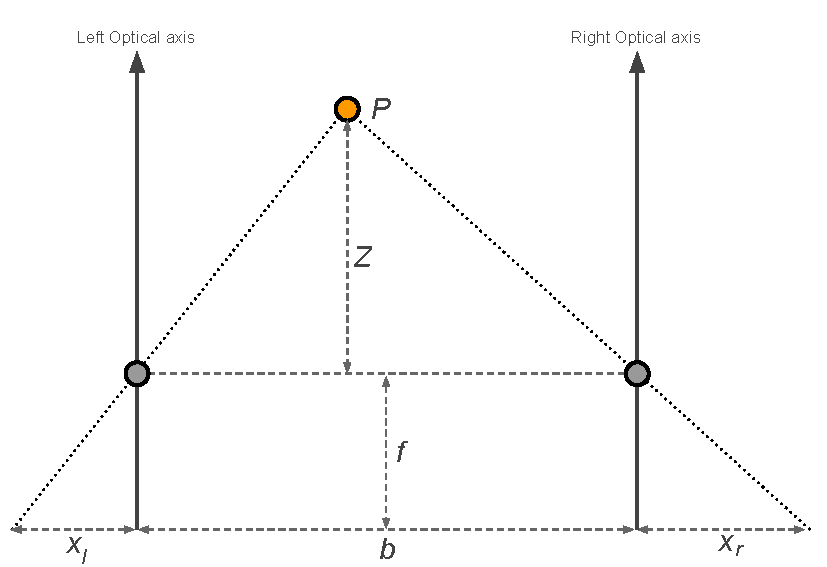
\includegraphics[width=0.8\textwidth]{images/depth-estimation-theory.pdf}
  \caption{Example of how the depth can be calculated}
\end{figure}

Figure \ref{fig:depth-theory} shows how the depth $z$ can be
triangulated. Given two corresponding points $x_l$ in the left image
and $x_r$ in the right, the disparity $d = x_l - x_r$, baseline
(distance between the cameras) $b$ and the focal length $f$, $z$ can
be calculated with the following formula:
\[
  \mathlarger{z = \frac{fb}{d}}
\]

Finding the corresponding points $x_{l}$ and $x_{r}$ is the main
challenge of all depth estimation approaches.


\section{Related Work}

Scharstein and Szeliski presents a very thorough taxonomy and evaluation of
many of the most known stereo correspondence algorithms in \cite{taxonomy}.
Most can be grouped into one of three types of algorithms: \textit{Feature-
based}, \textit{graph cuts} and \textit{Correlation-based}. Another way to
categorize them is by how they select what pixels are compared. \textit{Local}
algorithms only consider pixels in close proximity to the current pixel of
interest, while \textit{global} algorithms may consider pixels from anywhere
in the input. A third, lesser used category is \textit{semi-global}
algorithms, which consider every pixel up to the maximum search distance along
the scan line of the current pixel of interest.

Feature-based algorithms\cite{hannah74, marr-poggio79, nishimoto88} extract
features like edges, corners, circles and regions from the input images and
then find the disparity of the corresponding matches. These algorithms can be
fast, but are usually only able to produce sparse disparity maps, containing
values only near the features it could match. These algorithms have been in
use in mobile robotics for some time\cite{feature-based-robotics}, but is
unusable for applications like image-based rendering and view synthesis, which
need dense disparity maps, with values for all the pixels.

Graph cut algorithms\cite{markov98,boykov99,boykov04} are able to produce very
high quality disparity maps in terms of erroneous matches, but have a very
high computational cost. Even the fastest graph cut algorithms need seconds to
complete estimation on sub-VGA resolution inputs.

Lastly, there are correlation based algorithms. The fastest algorithms
mentioned in the taxonomy are all correlation based (the taxonomy only covers
algorithms producing dense disparity maps). Many implementations of
correlation-based algorithms exist and are used commercially. `Small Vision
Systems'\cite{svs98} and 'Point Grey'\cite{pg} sell devices capable of real
time depth estimation on lower resolutions, and Jet Propulsion
Laboratory\cite{jpl1, jpl2} has used the approach in mobile robotics. Most
correlation-based algorithms perform the correlation calculations using Sum of
Absolute or Squared Differences (SAD and SSD)\cite{faugeras93} or Normalized
Cross-correlation (NCC)\cite{ncc93} with a rectangular support region centered
around the pixel of interest.

\begin{figure}
  \centering
  \begin{subfigure}[b]{0.4\textwidth}
    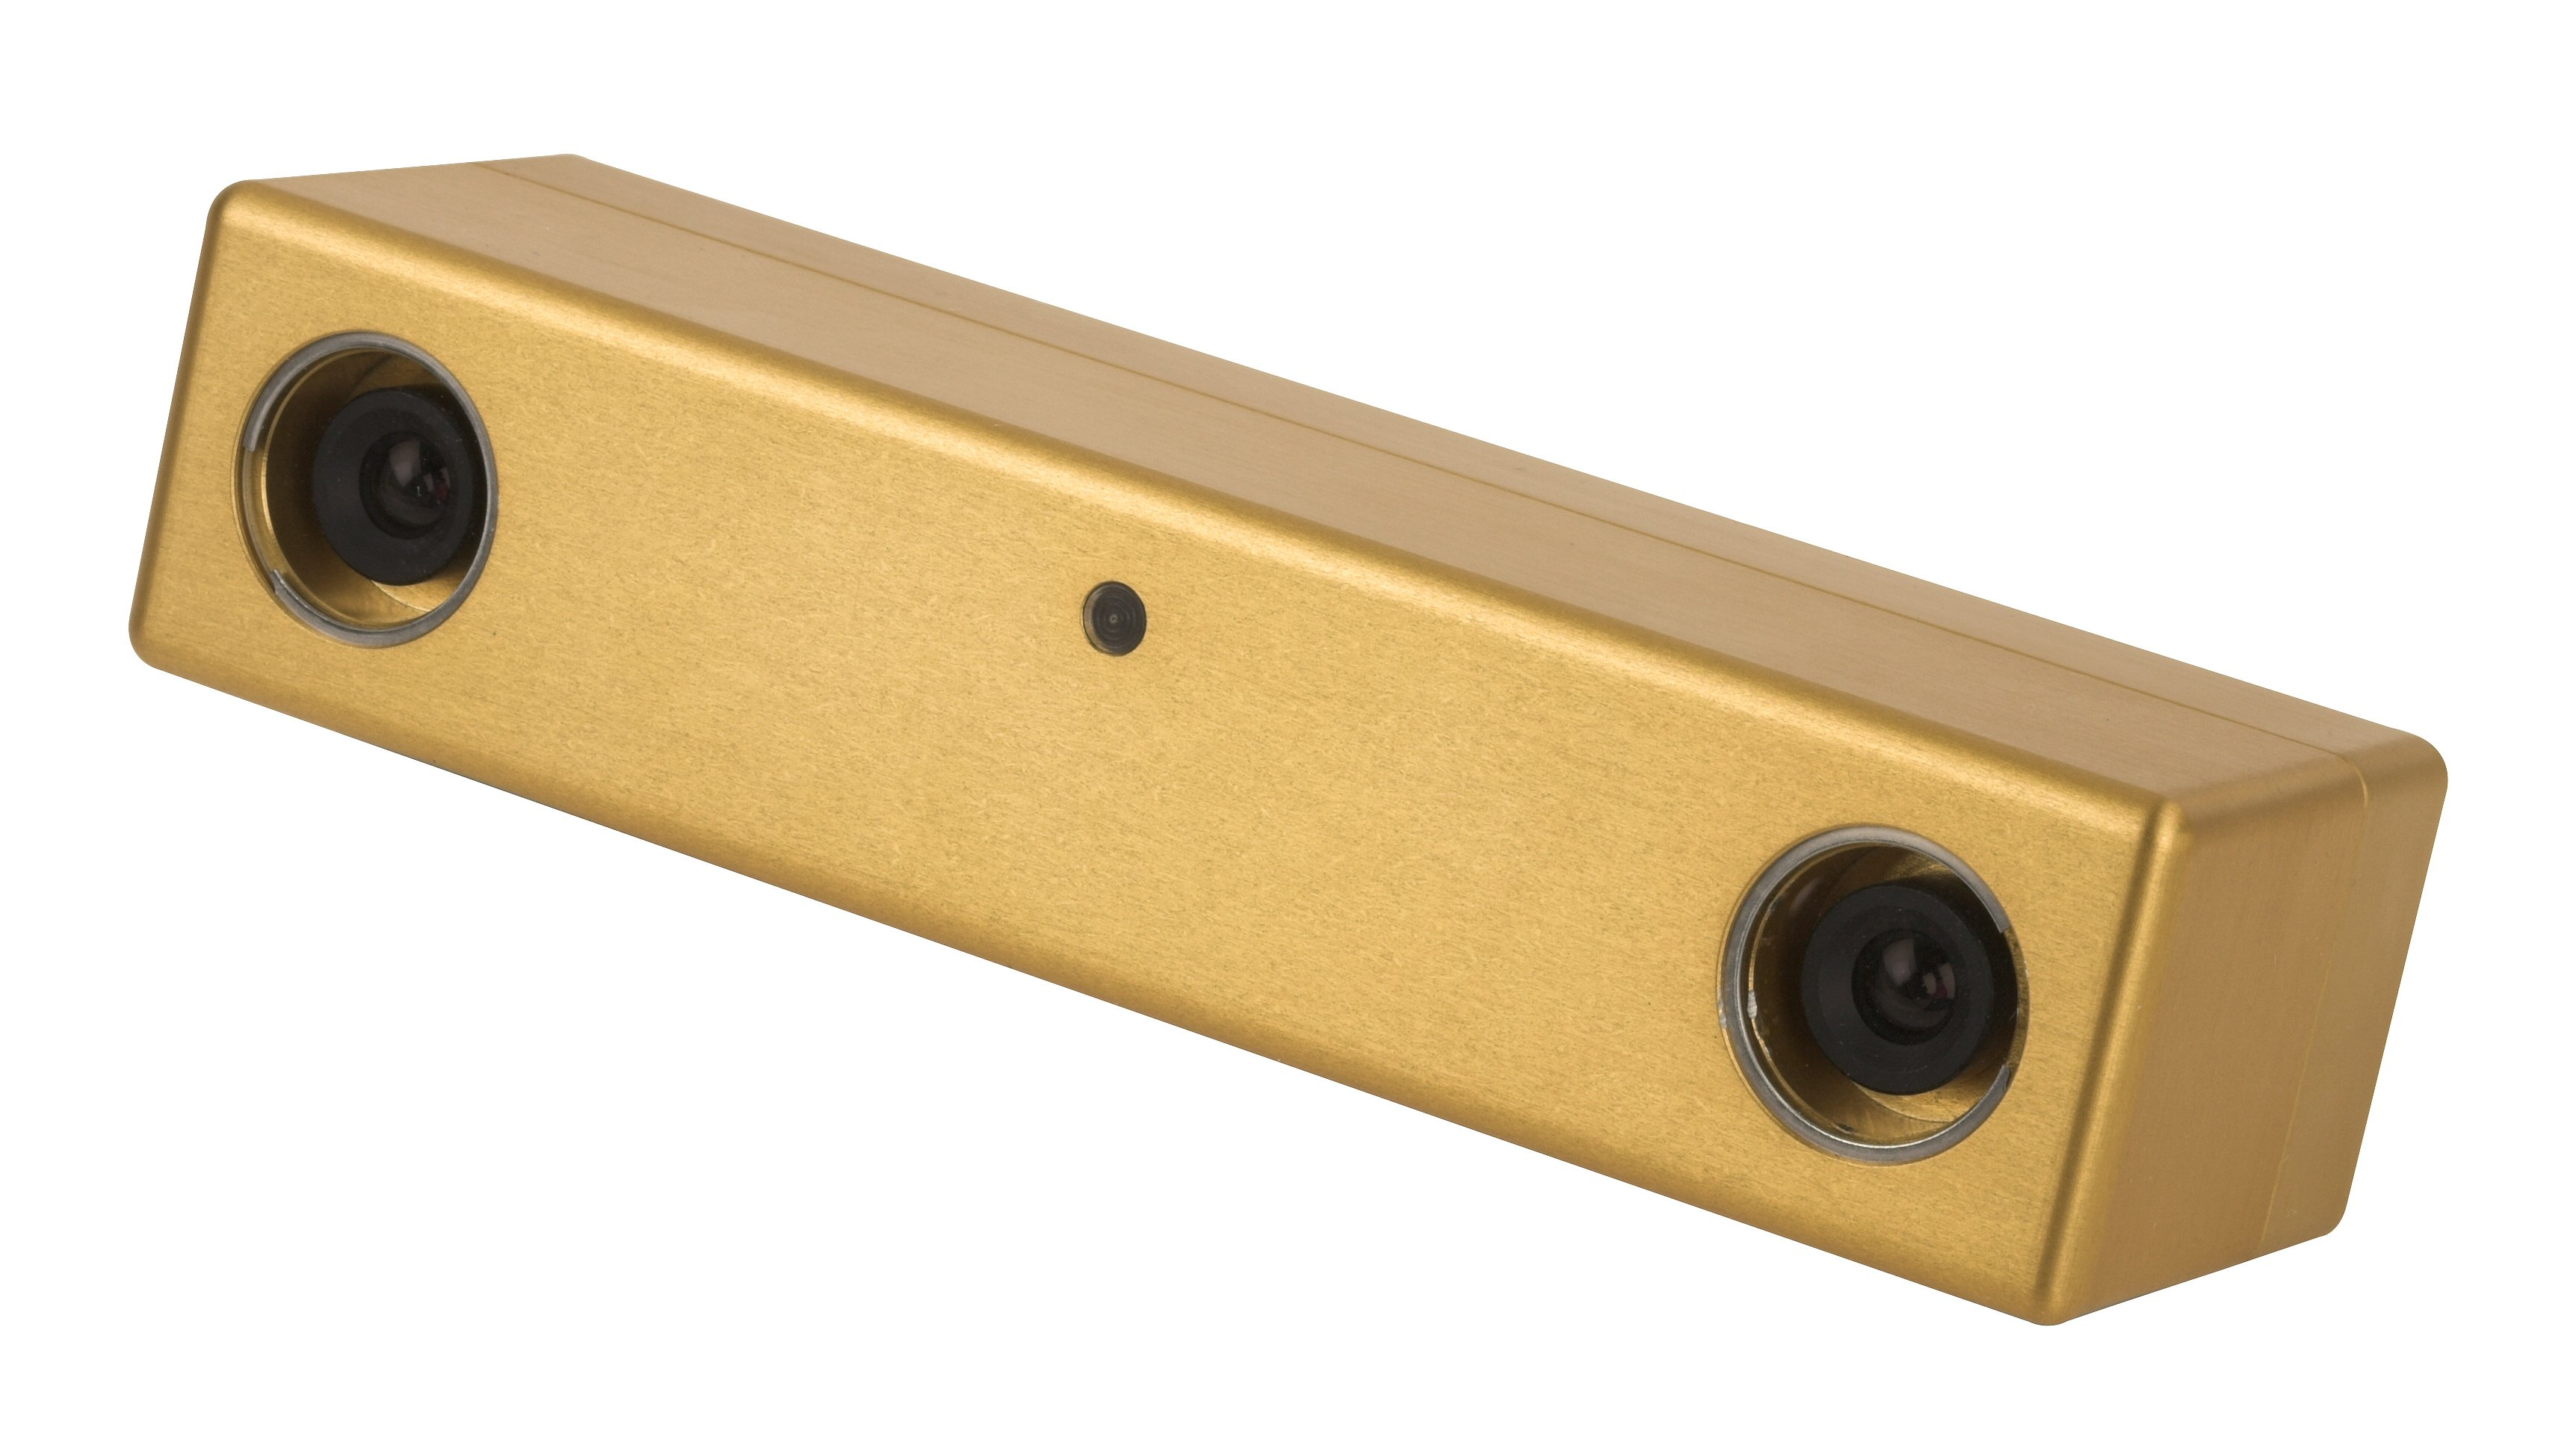
\includegraphics[width=\textwidth]{images/bumblebee2.jpg}
    \caption{Point Greys Bumblebee2 stereo camera}
  \end{subfigure}
  ~
  \begin{subfigure}[b]{0.4\textwidth}
    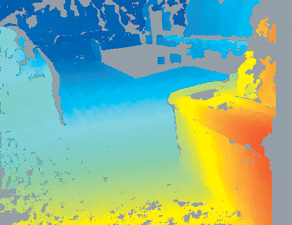
\includegraphics[width=\textwidth]{images/bumblebee_output.png}
    \caption{Bumblebee2 disparity map output}
  \end{subfigure}
\end{figure}


Regardless of approach, most algorithms perform the following four
steps in some way\cite{taxonomy}:

\begin{enumerate}
\item Matching Cost computation
\item Cost (support) aggregation
\item Disparity computation/optimization
\item Disparity refinement
\end{enumerate}

Not all approaches follow these steps rigorously. Feature-based approaches
usually have some pre-processing step that searches for features and then
perform the four steps on the areas around the extracted features. Graph cut
approaches usually skip the cost aggregation step, and instead search for a
value that minimizes a global cost function.

The correlation-based approach is what seems most likely to be able achieve
real time performance on high definition input, and will be the scope of this
thesis and the implementation.

\section{Block matching algorithm}

Of the correlation-based algorithms, \textit{block matching} algorithms seem
to achieve the best performance overall both in run time and disparity map
quality\cite{taxonomy}. Block matching algorithms get the name from
correlating windows (blocks of pixels), and not just single pixel or scanline
correlation. This window varies between algorithms, but is most often a square
window from $7\times7$ to $21\times21$ pixels. They may use adaptive windows
that changes shape on certain conditions, or other non-square shapes.



\subsection{Matching Cost calculation}
\label{sec:matchingcost}

The matching cost is a measurement of the similarity of pixel locations in the
input images. This calculation is typically done for all pixels, at all the
disparity hypotheses.

There are many ways to calculate this. Two of the simplest methods are
\textit{Absolute intensity differences} (AD):
\begin{equation}
  | I_L(x_L,y_L) - I_R(x_R,y_R) |
\end{equation}
and \textit{Squared intensity differences} (SD):
\begin{equation}
  (I(x_L) - I((x_r))^2
\end{equation}
These methods are very computationally quick to calculate, AD even
more so than SD.

Another well known matching technique is \textit{Birchfield and   Tomasi}'s
image sampling insensitive method (BT)\cite{bt}. Instead of comparing pixel
values shifted by integral amounts, BT compares each pixel in the reference
image against a linearly interpolated function of the other image. It has a
higher calculation cost, but has the benefit of alleviating input sampling
problems. As explained in the paper: $\hat{I}_R$ is first defined as the
linearly interpolated function between the sample points of the right
scanline, and measures how well the intensity at $x_L$ fits into the linearly
interpolated region surrounding $x_R$. The following quantity is defined:

\[ \mathlarger{\bar{d}(x_L, x_R, I_L, I_R) = \min_{x_R - \frac{1}{2}\  \le\  x\ \le \ x_R + \frac{1}{2}} | I_L(x_L) - \hat{I}_R(x) |} \]

Defining $\hat{I}_L$ similarly:

\[\mathlarger{
  \bar{d}(x_R, x_L, I_R, I_L) = \min_{x_L - \frac{1}{2}\  \le\  x\
    \le \ x_L + \frac{1}{2}} | \hat{I}_L(x) - I_R(x_R) |
}\]

a symmetric quantity is obtained. The dissimilarity $d$ between the pixels is
defined symmetrically as the minimum of the two quantities:

\begin{equation}
\label{eq:btd}
  \mathlarger{
    d(x_L,x_R) = \min \{\bar{d}(x_L,x_R,I_L,I_R),\  \bar{d}(x_R,x_L,I_R,I_L) \}
  }
\end{equation}

Since the extreme points of a piecewise linear function must be its
breakpoints, the computation of $d$ is straightforward. First, compute the
linearly interpolated intensity halfway between $x_R$ and its neighboring
pixel to the left:

\[
I^{-}_{R} \equiv{} \hat{I}_R ( x_R - \frac{1}{2}) =
\frac{1}{2}(I_R(x_R) + I_R(x_R - 1))
\]

and the analogous quantity:

\[
I^{+}_{R} \equiv{} \hat{I}_R ( x_R + \frac{1}{2}) =
\frac{1}{2}(I_R(x_R) + I_R(x_R + 1))
\]

Then, $I_{min} = \min\{I^{-}_{R},I^{+}_{R},I_{R}(x_R)\}$, and $I_{max}
= \max\{I^{-}_{R},I^{+}_{R},I_{R}(x_R)\}$

With these quantities defined, $\bar{d}$ can be calculated with:

\[
\bar{d}(x_L,x_R,I_,I_R) = \max\{0,I_L(x_L) - I_{max},I_{min} - I_L(x_L)\}
\]

along with its symmetric counterpart $\bar{d}(x_R,x_L,I_R,I_L)$.

For all approaches, a lower cost is a better match, where a cost of 0
means the left and right pixels are identical.

\subsection{Aggregation of Costs}
\label{sec:aggregatecost}

Single pixel matching is in most cases too ambiguous. Some kind of additional
information is needed. \textit{Local} algorithms sum up or average a small
neighborhood of costs into an aggregated cost, yielding a much better value
for comparison.

The simplest method is to sum the costs in a square window $w$ centered around
the pixel of interest. This method is known as \textit{Sum of Absolute
Differences} (SAD):

\begin{equation}
  \label{eq:sad}
  \mathlarger{\mathlarger{\sum}}_{i,j \in w} |I_L(i,j) - I_R(x + i, y + j)|
\end{equation}
or \textit{Sum of Squared Differences},
\begin{equation}
  \label{eq:ssd}
  \mathlarger{\mathlarger{\sum}}_{i,j \in w} (I_L(i,j) - I_R(x + i, y  + j))^2
\end{equation}
depending on which cost matching was used.

Aggregation with Birchfield \& Tomasi's image sampling insensitive method does
not have an equally catchy and widespread name, but the calculation is done in
the same manner using the equation \ref{eq:btd}:

\begin{equation}
  \label{eq:bt}
  \mathlarger{\mathlarger{\sum}}_{i,j \in w} \min\{
  d((x,y)_L,(x,y)_R), \ d((x,y)_L, (x+i,y+j)_R) \}
\end{equation}

Another slightly more complex technique is to use \textit{Adaptive
Windows}\cite{Okutomi and Kanade, 1992; Kanade and Okutomi, 1994;   Veksler,
2001; Kang et al., 2001)}. Instead of the fixed square windows mentioned
above, this approach computes costs in 5 smaller sub-windows arranged as shown
in figure t\ref{fig:adaptivewindow}. The final matching cost is determined by
the sum of costs from the center window, and the two surrounding windows with
the lowest sum of costs. This method handles object borders better than the
fixed windows at low resolutions, but on higher resolutions the smaller sizes
of the adaptive windows becomes insufficient\cite{gpugems}.


\begin{figure}
\label{fig:adaptivewindow}
  \setcounter{subfigure}{0}
  \centering
  \begin{subfigure}[b]{0.20\textwidth}
    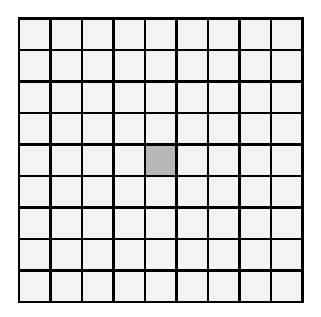
\includegraphics[width=\textwidth]{images/adaptive-windows-9x9.pdf}
    \caption{}
  \end{subfigure}
  ~
  \begin{subfigure}[b]{0.20\textwidth}
    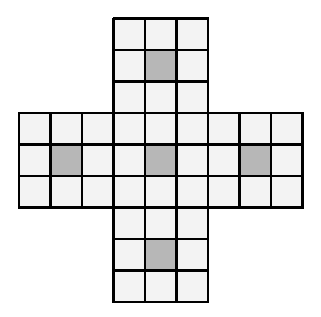
\includegraphics[width=\textwidth]{images/adaptive-windows.pdf}
    \caption{}
  \end{subfigure}
  ~
  \begin{subfigure}[t]{0.40\textwidth}
    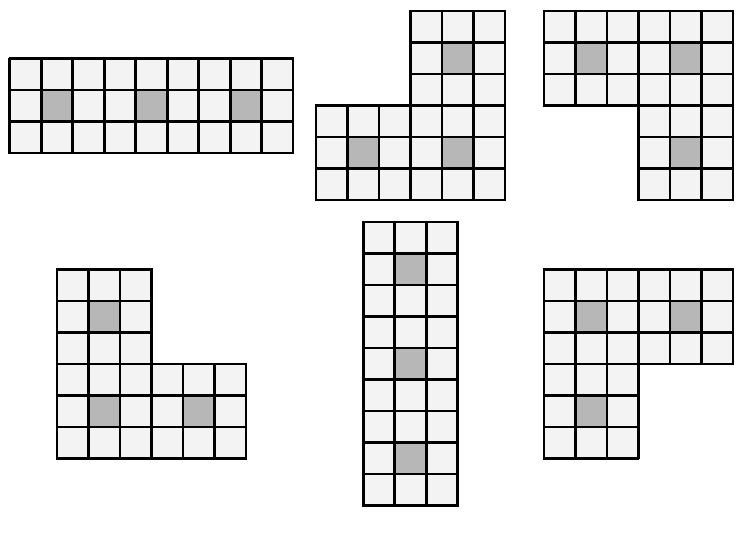
\includegraphics[width=\textwidth]{images/adaptive-windows-shapes.pdf}
    \caption{}
  \end{subfigure}
  \caption{(a) Fixed size window of 9x9 pixels; (b) adaptive windows,
    5 3x3 sub-windows; (c) possible combinations of center and 2
    adjacent windows}
\end{figure}


A lower aggregated cost is a better match, where a cost of 0 means the
left and right pixels and its neighborhood are identical.


\subsection{Disparity Selection}
\label{sec:disparity_selection}

The very simplest disparity selection strategy is the \textit{Winner-Takes-
All} (WTA), which is just a simple search for the lowest value among the
aggregated cost for each pixel. Not many other selection strategies for local
correlation-based algorithms have been proposed in research.

\subsection{Refinement}
\label{sec:refinement}

There are multiple disparity map refinements that can be applied. Of the most
common ones

Most depth estimation algorithms produce a disparity map of integer
disparities. Many applications such as robotics navigation and tracking do
fine with that level of quantization. However, for image-based rendering such
as \textit{Visual Hulls}\cite{torivar} and 3D-reconstruction, this level is
detail is detrimental to the quality of their output. This can be alleviated
by applying a sub-pixel refinement stage. Linear interpolation may be too
simple, but others have researched methods like including an iterative
gradient descent and fitting a curve to the matching costs at discrete
disparity levels \cite{Ryan et al., 1980; Lucas and Kanade, 1981; Tian and
Huhns, 1986;   Matthies et al., 1989; Kanade and okutomi, 1994, taxonomy}.

Applying a median filter to the disparity map removes high-intensity noise
caused by erroneous and spurious matches. Along an objects surface the
disparity is most likely going to be continuous, and blurring may even out
slightly-off matches.

Cross-checking eliminates unreliable matches. All depth discontinuities will
have occlusions, where a real world point is only visible on one of the
images, and will always produce an unreliable match. Cross-checking removes
these regions and marks them as invalid lets an application deal with it as it
sees fit.

The occlusions cross-checking has invalidated can be optionally be filled. For
the left disparity map, the background region immediately to the left of an
occlusion most likely stays constant up until the foreground object border.


\section{Summary}

Depth estimation is a vast field of research, and this chapter has barely even
glanced at the related work done. It has given a brief presentation of the
most common approaches, and discarded those that do not fit the goals of this
thesis. Block matching algorithms seem the most promising for a parallel
architecture, so it was explored and explained in further detail.
